\documentclass{article}

\usepackage{listings}
\usepackage{color}
\usepackage{courier}
\usepackage{amsmath}
\usepackage{graphicx}
\usepackage{float}
\usepackage[spanish]{babel}
\usepackage[utf8]{inputenc}
\usepackage{mleftright}
\usepackage{amsfonts}
\usepackage{hyperref}
\usepackage{csvsimple}
\usepackage{geometry}

\newcommand{\lnn}[1]{%
	\ln\left(#1\right)%
}

\newcommand{\lnb}[1]{%
	\ln\mleft(#1\mright)%
}


\title{PEC V - Física Computacional II}
\date{10-12-2023}
\author{Arturo Felipe Albacete Fernández}



\lstset{
	basicstyle=\footnotesize\ttfamily,
	breaklines=true,
	frame=tb,
	tabsize=4,
	columns=fixed,
	showstringspaces=false,
	showtabs=false,
	keepspaces,
	commentstyle=\color{red},
	keywordstyle=\color{blue}
}
\lstset{frame=single}

%\geometry{
%	 a4paper,
%	total={170mm,257mm},
%	left=15mm,
%	top=15mm,
%}

\begin{document}

% titulo
\maketitle
\newpage

% TOC
\tableofcontents
\newpage

% intro
%
% Introducción
%

\section{Introducción}

\paragraph{}
En este documento se encuentran redactadas las respuestas a la Prueba de Evaluación Continua 3. Se ha utilizado Python como lenguaje de programación y LaTeX para generar este documento.

\subsection{Sobre este documento}

\subparagraph{Estructura}
A cada pregunta se le ha dedicado una sección, en la que se intenta responder a los distintos puntos de la cuestión así como una explicación del código relacionado a la solución de dicha pregunta. En algunos casos, si una pregunta ya ha sido contestada en un apartado anterior, lo anotaré. 

\subparagraph{Código}
El código para esta (y otras PECs) lo estaré publicando en un repositorio git. Se puede acceder via:

\begin{lstlisting}[language=bash]
	git clone https://gitlab.com/aalbacetef/fisica-comp-II.git entrega-aalbacetef-fc-ii
\end{lstlisting}


Si se desea, puedo enviar por correo electrónico el código del proyecto en archivo comprimido (tar/rar/zip/7z/etc...).

Gran parte del código lo he puesto en el apéndice, pero recomiendo ver el repositorio git para poder leerlo más cómodamente.


\subsection{Ejecutar el código}

Para ejecutar el código es necesario tener Python instalado. He facilitado esto con el uso de Docker y un Makefile. Las instrucciones de como ejecutar se pueden encontrar en el README.md del repositorio.

\subsection{Información de contacto}

Si necesita contactarme por alguna razón, aparte de mi correo electrónico de la UNED, puede contactarme mediante:
\begin{itemize}
	\item \textbf{Email:} aalbacetef@gmail.com
\end{itemize}

\subsection{Afirmación de autoría del trabajo}

\paragraph{}

El firmante de este trabajo reconoce que todo él es original, de su única autoría, escritura
y redacción, y que allí donde han sido empleadas ideas o datos de otros autores, su
trabajo ha sido reconocido y ubicado, con suficiente detalle, como para que el lector
pueda consultar lo afirmado sobre él.
\newpage

% ejercicio A - regla del trapecio
\section{Ejercicio A - Regla compuesta del trapecio}

\subsection{Problema}

Calcule $C(\omega)$ y $S(\omega)$ para $\omega = 5$ utilizando las aproximaciones dadas por la regla
compuesta del trapecio usando un número de subdivisiones de

$$
n = 1, 2, 4, 6, 8, 16, 32, 64, 128, 256
$$

Indique, en cada caso, el número de evaluaciones necesarias de las funciones.

\subsection{Análisis}

\subsubsection{Derivación del método}

Dada una función $f(x)$, y un intervalo cerrado $I = [a, b]$, buscamos aproximar la integral definida: 

$$\int_{a}^{b} dx ~ f(x) $$


Empezamos dividiendo $I = [a, b]$ en $n$ subintervalos $I_n$ de tamaño 

$$
\Delta x = \frac{b - a} {n}
$$.

Esto nos da un conjunto $ X = \{ x_k \}$ de $n + 1$ puntos: 

$$
x_k = a + k \Delta x  = a + \frac{ k}{n}(b-a)
$$

y el valor de $f(x)$ en cada punto es:

$$
f_k = f(x_k) = f(a + \frac{ k}{n}(b-a) )
$$


Entre cada punto $x_k$ y $x_{k+1}$ intentamos aproximar el área bajo la curva $f(x)$ por un trapecio de base $x_{k+1} - x_k = \Delta x$, lado menor $y_k$ y lado mayor $y_{k+1}$. Esto nos da un área de tamaño:

\begin{align*}
	A_k 
	&= A_{\Box_k} + A_{\triangle_k} \\
	&= (f_k \Delta x ) + \frac{1}{2}(f_{k+1}-f_k)(\Delta x) \\
	&= (\Delta x)( f_k + f_{k+1} )\frac{1}{2}
\end{align*}

\newpage 

La integral se puede aproximar entonces por:

\begin{align*}
	\int_{a}^{b} dx ~ f(x)
	&\approx \sum_{k = 0}^{n - 1} (\Delta x)( f_k + f_{k+1} )\frac{1}{2} \\
	&= \frac{\Delta x}{2} \sum_{k = 0}^{n - 1} ( f_k + f_{k+1}) \\
	&= \frac{\Delta x}{2} (\sum_{k = 0}^{n - 1}  f_k + \sum_{k = 0}^{n - 1} f_{k+1}) \\
	&= 
	\frac{\Delta x}{2}
	(
	f_0 + \sum_{k = 1}^{n - 1}  f_k 
	+ \sum_{k = 0}^{n - 2} f_{k+1}
	+ f_n
	) \\
	&= \frac{\Delta x}{2}(f_0 + f_n  + 2 \sum_{k = 1}^{n - 1}  f_k )
\end{align*}


Por ende: 

\begin{equation}
\boxed{\frac{\Delta x}{2}(f_0 + f_n  + 2 \sum_{k = 1}^{n - 1}  f_k )}
\end{equation}



\subsubsection{Implementación}

El método se puede ver implementado en \ref{code:trapezium}


\newpage 

\subsection{Resolución}

El código que resuelve el ejercicio se puede ver en \ref{code:ex1}. 

Obtenemos la siguiente figura:

\begin{figure}[H]
	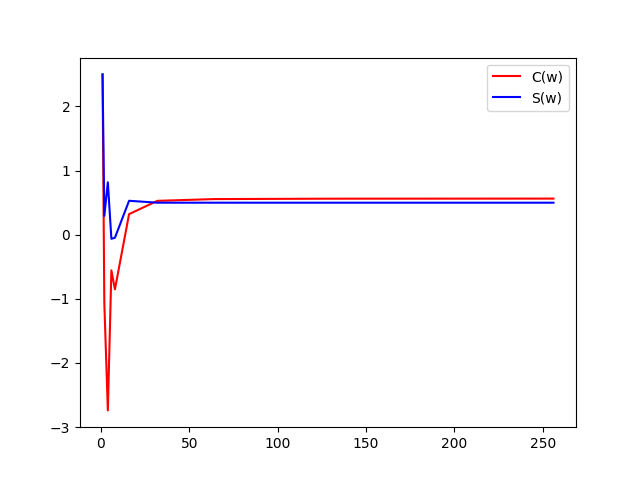
\includegraphics[width=\linewidth]{figures/ex1.png}
	\caption{Gráfica de C($\omega$) y S($\omega$) usando la regla del trapecio por cada $n$.}
	\label{fig:c_s_subdiv}
\end{figure}


\begin{table}[H]
	\centering
	\csvreader[
	tabular=|c|c|c|,
	table head=\hline \textbf{n} & \textbf{C($\omega$)} & \textbf{S($\omega$)} \\\hline,
	late after last line=\\\hline,
	]{data/c_s_subdivs.csv}{}{\csvlinetotablerow}
\end{table}

\paragraph{Discusión}

Vemos pues que los valores convergen, siendo bastante estables a partir $n = 32$.

\newpage 


% ejercicio B - método de romberg
\section{Ejercicio B - Método de Romberg}


\subsection{Problema}

Utilizando los resultados del apartado a), realice la extrapolación de Romberg para obtener una mejor aproximación numérica de las dos integrales de Fresnel. Indique cuántas evaluaciones de las funciones se requieren.


\subsection{Análisis}


\subsubsection{Extrapolación de Richardson}

La extrapolación de Richardson es un método que pertenece a la familia de aceleración de series.

Se puede aplicar cuando el error de una aproximación sigue la forma: 

$$
O(x^p) = \sum_{k=p} a_k (x - c)^k
$$

Dada una constante que nos interesa aproximar, como por ejemplo:

$$
m = \int_{a}^{b}  f(x) dx
$$

planteamos una aproximación $L_i(h)$, función del valor del paso discretante del dominio $I = [a, b]$. Le daremos la forma: 

$$
m = L_j(h) + \sum_{k = j}a_k h^k
$$

El error es la suma y es de orden $O(h^j)$.

Si reducimos el paso por un factor de $\frac{h}{2}$ y manipulamos algebraicamente obtenemos una nueva aproximación en el que el término de orden $O(h^j)$ es eliminado.


\subsubsection{Método de Romberg}

El método de romberg se basa en obtener una aproximación mejor combinando la regla del trapecio compuesto con la extrapolación de Richardson.

\subsubsection{Implementación}

La implementación del método se puede ver en \ref{code:romberg}

\subsection{Resolución}


El código que resuelve el ejercicio se puede ver en \ref{code:ex2}. 

\paragraph{Valores} Los resultados se han compilado en una tabla.


\begin{table}[H]
	\centering
	\csvreader[
	tabular=|l|l|l|,
	table head=\hline \textbf{fn} & \textbf{Valor} & \textbf{Num. Evals} \\\hline,
	late after last line=\\\hline,
	]{data/romberg_c_s.csv}{}{\csvlinetotablerow}
\end{table}


\newpage 

% ejercicio C - cuadratura de Gauss
\section{Ejercicio C - Cuadratura de Gauss}


\subsection{Problema}

Calcule $C(\omega)$ y $S(\omega)$ para $\omega = 5$ utilizando la cuadratura gaussiana de $64$ puntos. En el Plan de Trabajo del curso virtual (Tema 5), se da un fichero con dos columnas de datos. La primera columna son las raíces del polinomio de Legendre de grado 64 en el intervalo $[-1, 1]$ y la segunda son los pesos (o factores de ponderación) correspondientes para la cuadratura gaussiana.

\subsection{Análisis}

El problema se trata de usar la forma de Gauss-Legendre, pero con una traslación del intervalo $[1, 1]$ al intervalo $[a, b]$.

\paragraph{Cuadratura de Gauss}

La cuadratura de Gauss-Legendre aproxima la integral de una función sobre un intervalo $[-1, 1]$ usando factores de ponderación $(w_i)$ y polinomios ortogonales con raices $x_i$.

Esto tiene la forma:

$$
\int_{-1}^{1} dx ~ f(x) 
\approx \sum_{i} w_i f(x_i)
$$


\paragraph{Traslación}
Para hacer una traslación de una cuadratura de Gauss:

$$ \sum w_i f(x_i) = \int_{-1}^{1} dx ~ f(x) $$ 

Se modifican los parámetros de la siguiente forma: 

$$
\int_{a}^{b}dx~ f(x) = \frac{b - a}{2} \int_{-1}^{1} dx ~ f( \frac{b-a}{2} x + \frac{a + b}{2})
$$

Y usando la aproximación de Cuadratura de Gauss:

\begin{equation}
\int_{a}^{b}dx~ f(x) \approx
\frac{b - a}{2}
\sum_{i}w_i f(\frac{b-a}{2} x_i + \frac{a + b}{2} )
\end{equation}



\subsubsection{Implementación}

La implementación del método se puede ver en \ref{code:gauss_quad}


\subsection{Resolución}


El código que resuelve el ejercicio se puede ver en \ref{code:ex3}. 

\paragraph{Valores} Los resultados se han compilado en una tabla.


\begin{table}[H]
	\centering
	\csvreader[
	tabular=|c|c|c|,
	table head=\hline \textbf{fn} & \textbf{Valor} \\\hline,
	late after last line=\\\hline,
	]{data/gauss_quad_c_s.csv}{}{\csvlinetotablerow}
\end{table}




\newpage

% ejercicio D - comparación de las aproximaciones
\section{Ejercicio D - Error de la aproximación}

\subsection{Problema}

Recoja en una tabla de datos los puntos $x_i \in [0, 5]$ utilizados en la aproximación numérica de las integrales de Fresnel cuando se utiliza la cuadratura gaussiana de 64 puntos del apartado c) y los $x_i$ necesarios para la aproximación dada en el apartado a), cuando se utiliza la regla compuesta del trapecio con n = 64. (Si prefiere, además de la tabla de datos puede realizar una representación gráfica). Calcule los errores cometidos con estos dos métodos en relación a las estimaciones más exactas de las integrales, es decir, las obtenidas con la extrapolación de Romberg en el apartado b. Discuta los resultados.

\subsection{Resolución}


El código que resuelve el ejercicio se puede ver en \ref{code:ex4}. 

\subsubsection{Puntos $x_i$}

La tabla de puntos se puede ver en \ref{ex4:table}. Una figura de los puntos $x_i$ se puede ver a continuación. 

\begin{figure}[h!]
	\centering
	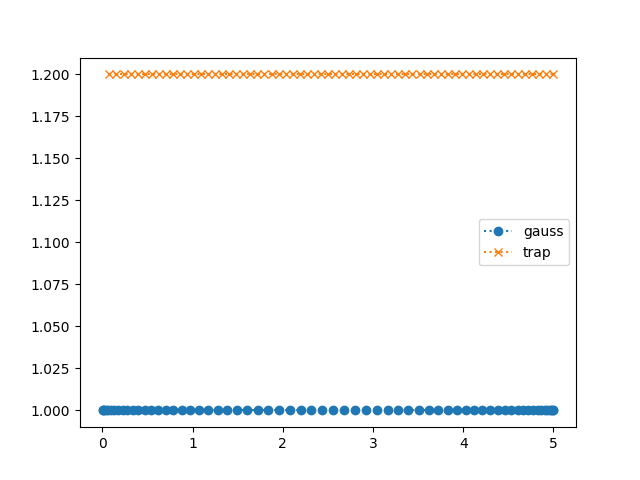
\includegraphics[width=0.8\linewidth]{figures/gauss_trap_xi.png}
	\caption{Gráfica los puntos $x_i$ de la aproximación de Caudratura de Gauss y Regla Compuesta del Trapecio.}
	\label{fig:gauss_trap_xi}
\end{figure}

\paragraph{Discusión} 
La principal diferencia entre los dos conjuntos de $x_i$ es que en el caso de la regla compuesta del trapecio se particiona el intervalo de forma uniforme, mientras que en la cuadratura gaussiana los puntos tienen mayor densidad en los extremos del intervalo.

Esto queda ilustrado muy claramente en la siguiente figura:
\begin{figure}[h!]
	\centering
	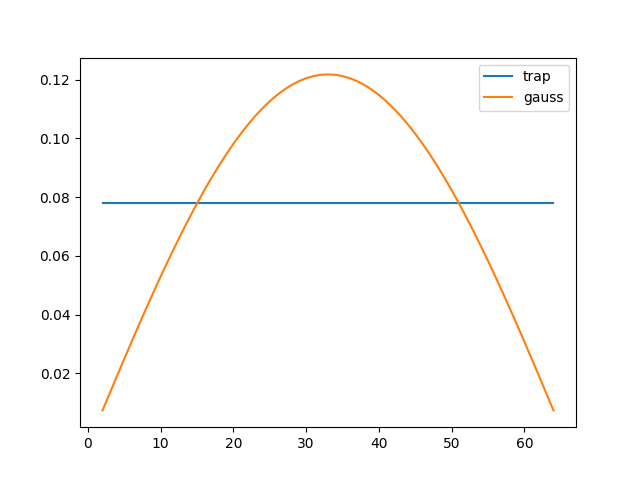
\includegraphics[width=0.8\linewidth]{figures/gauss_trap_diff_xi.png}
	\caption{Diferencia entre los puntos $x_i - x_{i-1}$ de las dos aproximaciones.}
	\label{fig:gauss_trap_diff_xi}
\end{figure}

\subsubsection{Errores}

El error absoluto $v_{approx} - v_{romberg}$ en las aproximaciones, con respecto al valor dado usando el método de Romberg es: 

\begin{table}[H]
	\csvreader[
	tabular=|c|l|l|,
	table head=\hline \textbf{fn} & \textbf{C($\omega$)} & \textbf{S($\omega$)} \\\hline,
	late after last line=\\\hline,
	]{data/abs_error_approx.csv}{}{\csvlinetotablerow}
\end{table}

Y el error relativo, dado por $ 100 * \frac{|err_{abs}|}{v_{romberg}}$: 
\begin{table}[H]
	\csvreader[
	tabular=|c|l|l|,
	table head=\hline \textbf{fn} & \textbf{C($\omega$) (en \%)} & \textbf{S($\omega$) (en \%)} \\\hline,
	late after last line=\\\hline,
	]{data/rel_error_approx.csv}{}{\csvlinetotablerow}
\end{table}

\paragraph{Discusión}
Como vemos, de las dos aproximaciones, la aproximación de cuadratura gaussiana tiene menor error que la de la regla compuesta del trapecio, aunque las dos tienen errores bastante aceptables en este caso.
\newpage

% apendice
\section{Apéndice}

\subsection{Código linalg}
\label{code:linalg}

\lstinputlisting[language=Python]{../../code/methods/linalg.py}


\subsection{Código datos}
\label{code:datos}

\lstinputlisting[language=Python]{../../code/pecs/pec4/data.py}

\subsection{Código Ejercicio C}
\label{code:ex3}

\lstinputlisting[language=Python]{../../code/pecs/pec4/ex3.py}

\subsection{Código Ejercicio D}
\label{code:ex4}

\lstinputlisting[language=Python]{../../code/pecs/pec4/ex4.py}

\subsection{Código Ejercicio E}
\label{code:ex5}

\lstinputlisting[language=Python]{../../code/pecs/pec4/ex5.py}

\subsection{Código Ejercicio F}
\label{code:ex6}

\lstinputlisting[language=Python]{../../code/pecs/pec4/ex6.py}

\subsection{Código Ejercicio G}
\label{code:ex7}

\lstinputlisting[language=Python]{../../code/pecs/pec4/ex7.py}
\newpage



\end{document}
